\section{The Autoencoder}
\subsection{Deep Neural Networks}

To clearly explain what an Autoencoder is, we must first lay the foundations of one of its core concepts: Deep Neural Networks. DNN constitute the basis of Deep Learning and they have proven themselves to be complex enough to tackle many of the data challenges of today. \par

\begin{figure}[H]
\begin{subfigure}{0.65\linewidth}  
 \centering
  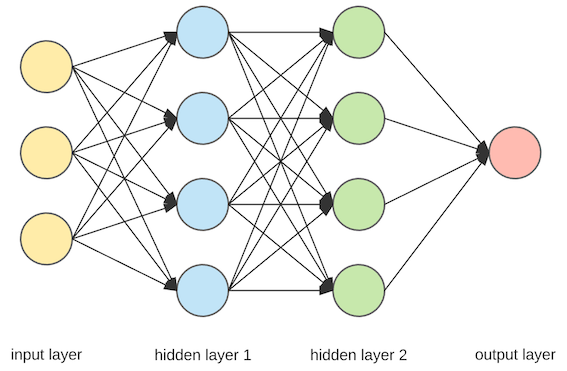
\includegraphics[width=\linewidth]{Figuras_tfg/Figure2_tfg}
  \caption{Basic depiction of a simple DNN composed by two hidden layers and a single 2-input/1-output system.}
  \label{fig:fig2a} 
\end{subfigure}

\begin{subfigure}{0.65\linewidth} 
  \centering
  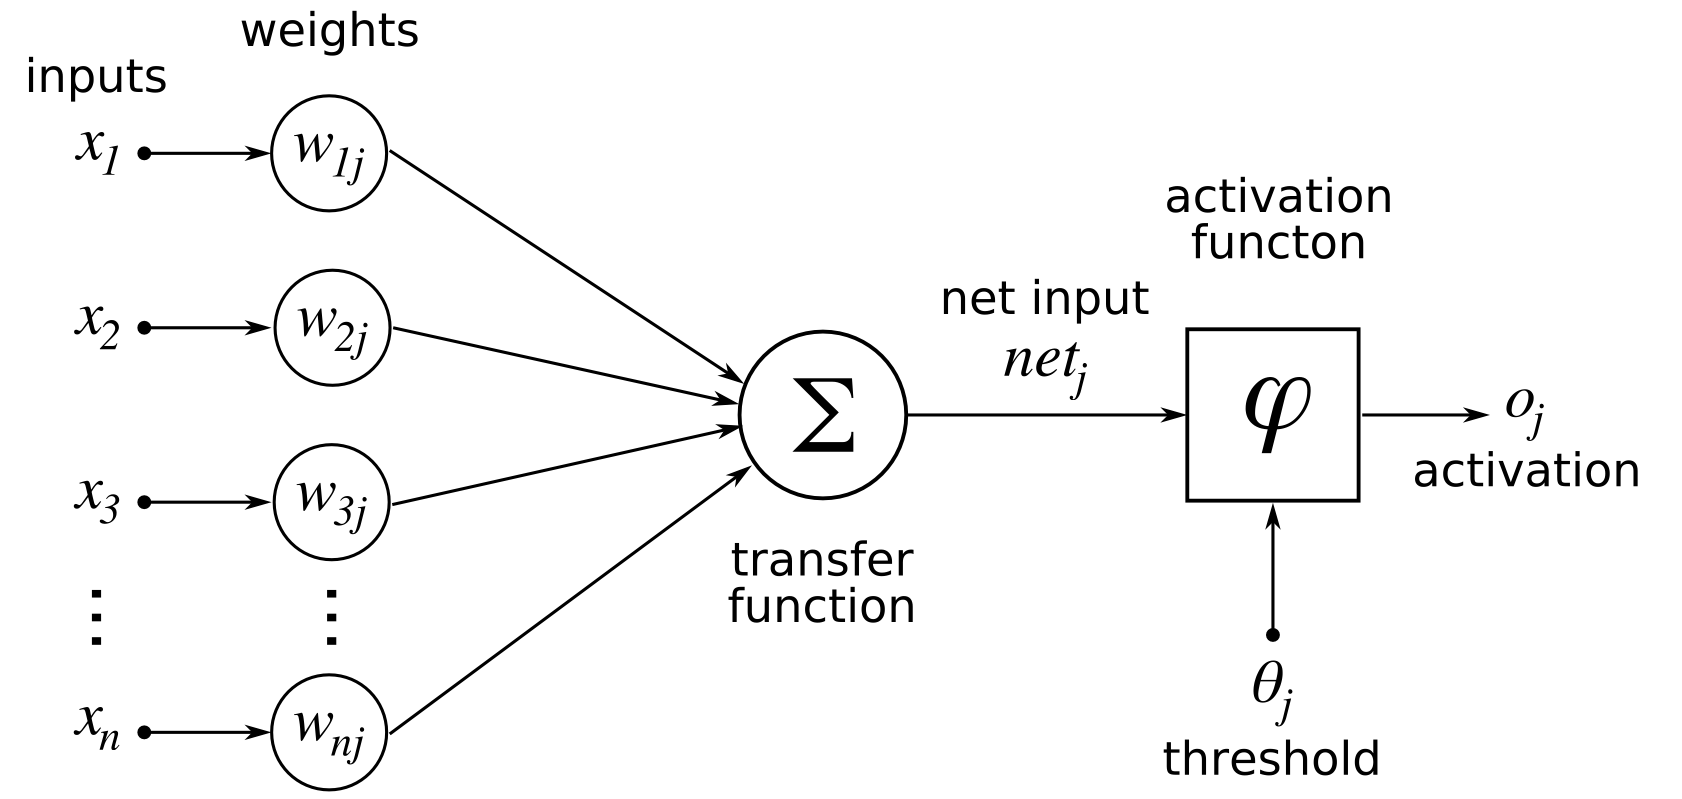
\includegraphics[width=\linewidth]{Figuras_tfg/ArtificialNeuronModel_english.png}
  \caption{Normal architecture of an artificial neuron.}
  \label{fig:fig2b} 
\end{subfigure}
  \caption{Basic depiction of a simple DNN composed by two hidden layers and a single 2-input/1-output system.}
 \label{fig:fig2}
\end{figure}

By analysing Figure2a, it can be noted that DNNs are comprised of multiple layers of units (or neurons) with a relatively small computing power which is calculated using the weights from previous layers combined with an activation function as seen on and \ref{fig:fig2}. It also has an input (usually denoted as X) which is feed-forwarded to the hidden layers in the network and subsequently transformed into an output (commonly denoted as Y). 

\begin{equation}\label{eq:artificial neuron}
Output = f( bias_j + \sum_{i = 0}^{n} w_{i}*x_i ) 
\end{equation}


Neurons inside of the network can be modelled according to different types, although in this report we will be only taking into account two of them: the sigmoid $f(x) = \frac{1}{1 - e{-x}}$ (Figure a) and the relu $f(x) = max(0,x)$(Figure b) neurons. I chose to use this type of neurons because their activation functions are excellent for minimizing the reconstruction loss inside of the autoencoder. \newline

\begin{figure}[H]
 \begin{minipage}{.5\textwidth}
        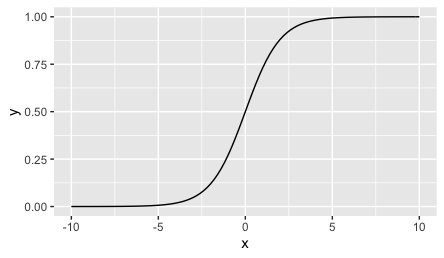
\includegraphics[scale=.5]{Sigmoid_function}
 \end{minipage}%
 \begin{minipage}{.5\textwidth}
        \begin{flushright}
               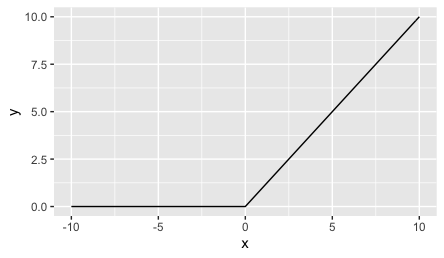
\includegraphics[scale=.5]{Relu_function}  
        \end{flushright} 
    \end{minipage}  
    \caption{The left graph represents a Sigmoid function, while on the right there is a Relu function}
 \label{fig:fig3}
\end{figure}

As it can be seen on Figure\ref{fig:fig3} , the Relu function has a relatively simple representation, which makes it less computationally expensive when compared with the Sigmoid. The Sigmoid function is also very useful since it takes values between 0 and 1, which makes it specially useful when we want to place a classifier as the next task after the transformation.\par 

Once a certain DNN structure has been activated, the neurones inside of the network will start to propagate the information through it in a non-linear manner in order to try to achieve a given stablished task, which in our particular case consists in transforming the representation of our input into a smaller but informationally more compressed form. Other experts can use the same principles to achieve other goals including decision-making, visualisation,....etc.\par

\subsection{Information Bottleneck Principle}

The architecture of the Autoencoder is based upon the IB, a method proposed in [paper which mentions it] whose principle relies on extracting the relevant information that an input random variable X contains about another output random variable Y. If we assume that there is some type of statistical dependency between X and Y, the relevant information can be defined as I(X;Y).\par

If we want to obtain the optimal representation of X we would want to capture the relevant information of X that contributes to an accurate prediction of Y. This term is known as the (minimal sufficient statistics), or simply just the mapping of X that retains I(X;Y).\par

During the learning process, and as depicted in figure (DNN self-explanatory figure), DNN only have access to the information that has been transferred to them via the previous layers of the system. This has a big effect on out network: the information not processed on the last immediate layer is essentially lost. This is the main reason why every layer should attempt to maximise I(Y;hi) while trying to minimise the I (hi-1;hi). Here, it is important to consider then that we want to reduce the length of the layer to the minimum possible without affecting the the predictive features of our model.

Each layer of our model should require shorter descriptions than the previous ones, being the first one with the longest description and the least compression. It must also be noted that every model will require a different set of layers an architecture to fit its computational needs to the optimal level.

\subsection{The Autoencoder Architecture}

Applying the concepts introduced on both previous sections (the two sections appearing before this one, when  i figure the final numbers ), the autoencoder comes as a mixture of them. Figure [] below presents it as a three part structure: A encoder, the middle layer and finally the decoder. \par

\begin{figure}[H]
 \centering
  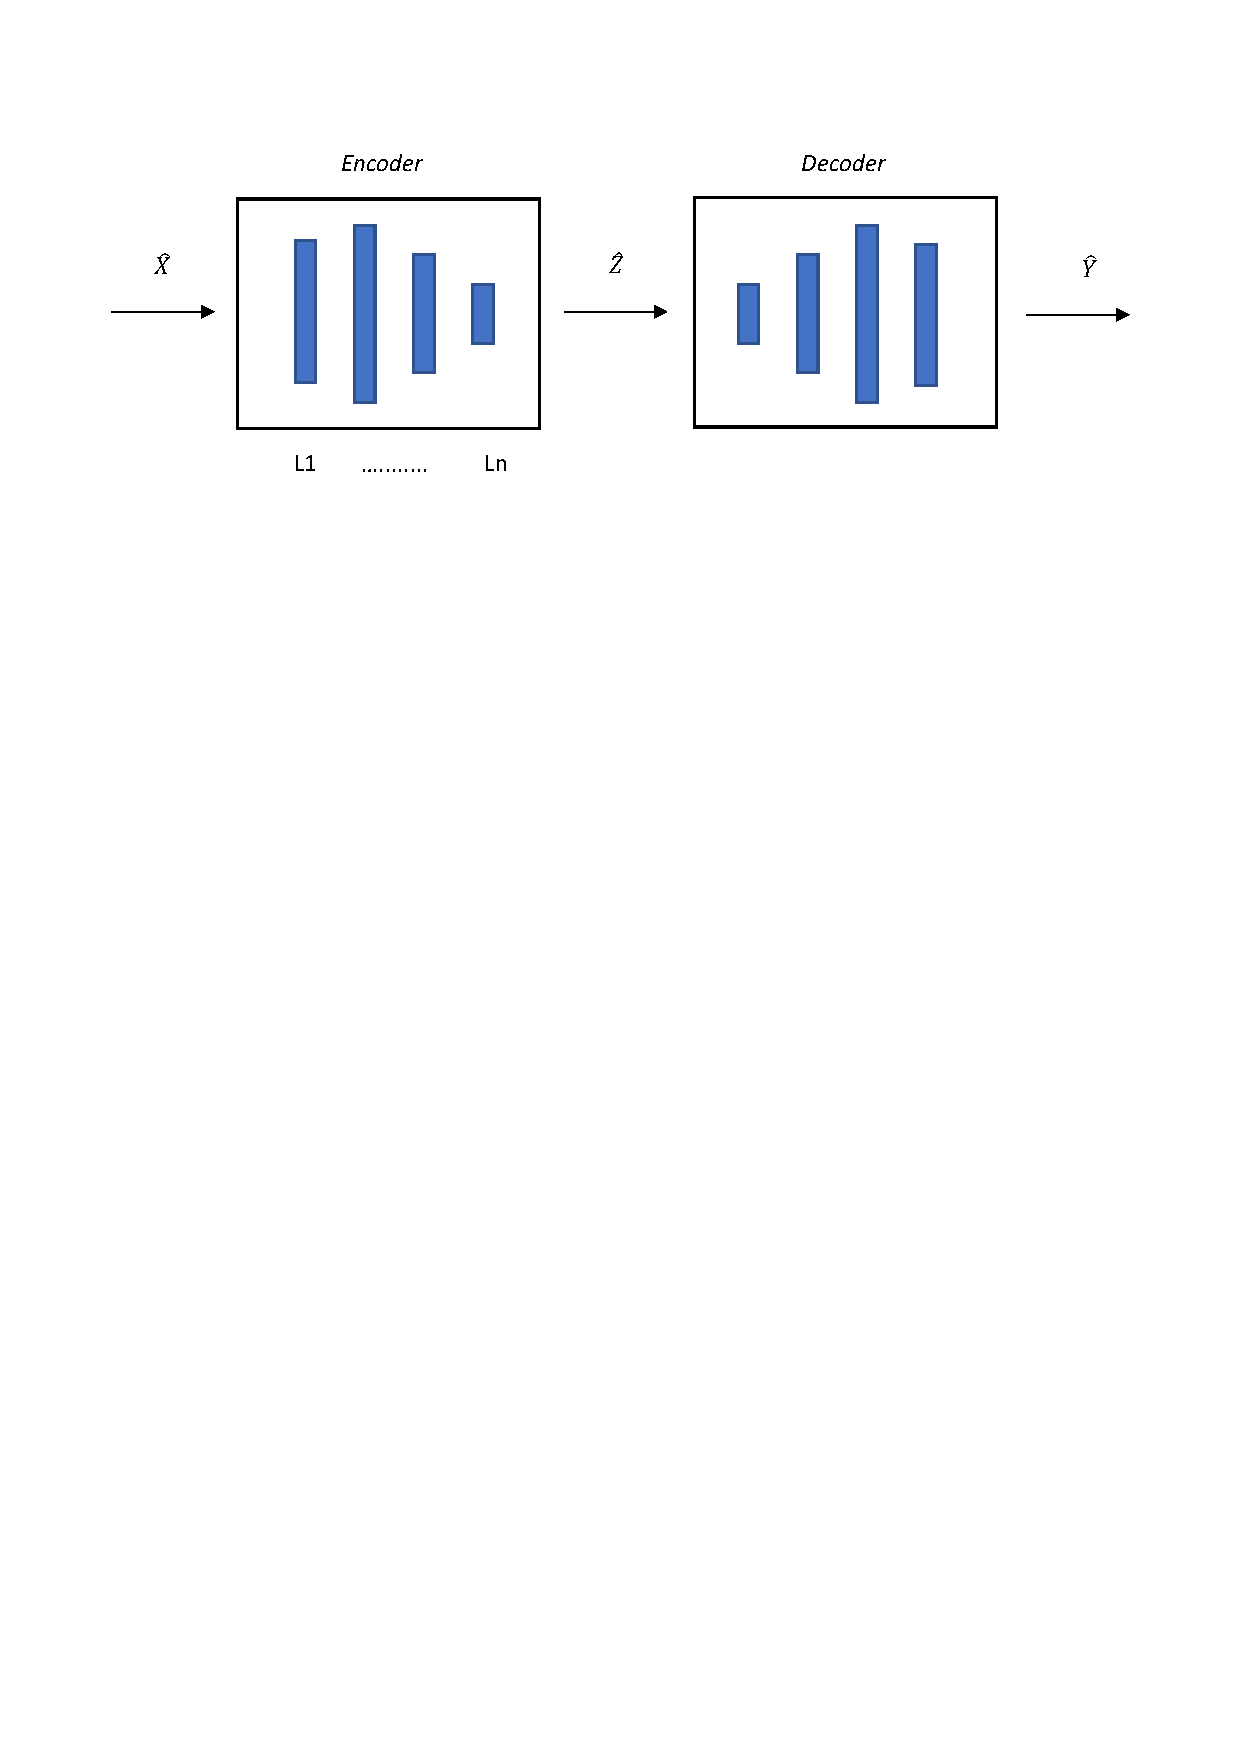
\includegraphics[width=16cm]{Figuras_tfg/Figura_autoencoder}
  \caption{Taking into account the Figure \ref{fig:fig1a}, this diagram depicts the inside of the transformation box. Both the Encoder and the Decoder have symmetric shapes, as well as an expansion layer (the second one in the encoder, the previous one in the decoder) whose goal is to separate the qualities of our data as sort of a preparation for the compression.}
 \label{fig:figure_autoencoder}
\end{figure} 

The theory of the autoencoder has been around since the 1980s (put as a reference the article where it is first presented). As seen in Figure[], the autoencoder's goal is not only to copy the input data and then transmit it through the network, but to retain the most important features of the data fed to it and to try to optimise the process of learning them. For the purpose of my research, I will only be considering the back-propagated autoencoders, although it must be noted that other variances of them exist, such as the recirculated autoencoders. \par

In our case, we will be also using an undercomplete autoencoder. Most of the types an autoencoder is employed, it is usually more interesting to focus on its data compression capabilities rather than trying to copy the input onto the output. That is why we want to force the autoencoder to provide us with a smaller dimension on the input data X in the output on the encoder, which for the purpose of this report we will denominate as Z. The learning process, as described in (paper where i got the equation from) tries to minimise the given equation: \par

\begin{equation}\label{eq:artificial neuron}
L(x,g(f(x)))
\end{equation}
The L function is a loss function, which penalises $g(f(x))$ for being dissimilar from $x$.

One thing to take into account when designing an autoencoder is that giving too much capacity to its layers can be counterproductive to the learning task. This means that when given too much capacity to work with they will tend to learn to avoid extracting information and rather to just copy the information, which is an undesirable outcome. On the other hand, trying to set an encoder to code the input signal into a single dimension could result in the loss of valuable information. Even with a very powerful decoder a very optimised autoencoder will struggle to perform this task, specially when introducing very big sets data as the input. \par

Taking into account this description, the general rule to design it is just by using trial and error. As we will see on Section3, where I will be discussing the implementation of the autoencoder, you can try different setups to reach the optimum middle layer size which accomplishes that there is no trade-off between augmenting its size and keeping its actual capabilities. The Tensorflow python tool provides us with the accuracy and loss variables that the autoencoder is generating on each training epoch to check if your architecture is fulfilling your requirements. For the purpose of this report, we will not only taking into account those parameters, but we will also be using a tool to ensure that it transfering the higher quantity of information possible: The entropy triangle.

\subsection{The Entropy Triangle}
\subsubsection{Introduction}

In the previous section I have talked about how accuracy can be used to asses the validity of our model. In reality, the accuracy value can be somewhat misleading depending of the task that we are implementing it to check if we are carrying out our data analysis correctly. This statement is specially true when talking about Classification.\par

The usage of data classification has greatly improved in the past years. Nowadays, there are multiple papers discussing how it can be used in a wide range of topics, from the medical field to the face recognition task. That is why it is specially important to correctly address the scope of your task and how accurately does your model predict in your pre-defined scenarios.\par

\begin{figure}[H]
 \centering
  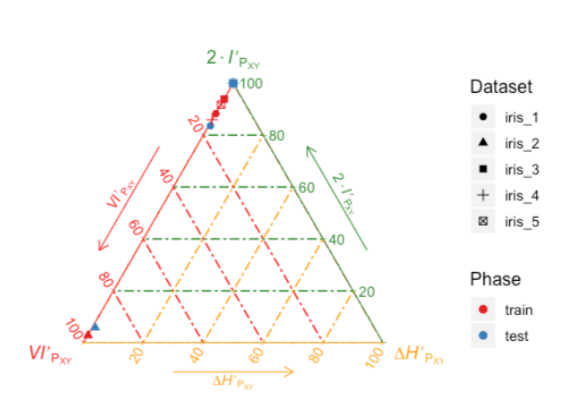
\includegraphics[width=15cm]{Figuras_tfg/Example_ET}
  \caption{Example of use of a typical Entropy Triangle. In this case, a Knn classification method is being tested in the triangle.}
 \label{fig:figure_example_et}
\end{figure} 

The real question comes when you have your results and you try to wrap your mind around them. In [paper donde se discute ese tema] a very important reality is shown: the accuracy performance criterion is a very intuitive but ineffective tool. Another highly important concept is introduced here: the accuracy paradox.\par  

The accuracy paradox shows some of the defects that classifiers have been presenting for a long time now . For example, in some cases predictive classifiers which have given a lower accuracy power have also proven to display a higher predictive accuracy that other with a higher accuracy. The reason being most of the times is that we have trained our classifier with a single class that contains the majority of the data. In those cases, our classifier will just assign all of the input values to belong to the majority class since that is where the greater probability lies upon. This one is a very easily identifiable case of an imbalanced training data set. Moreover, since most of the times our data is gathered in controlled conditions, we risk the problem of this issue showing up more than we would wish to.\par

Once it is realised that the methods previously employed can lead to disingenuous results, a new realisation arrises: there is a need for a better measure of the classifier. As seen in, the Entropy Triangle and its features show some numeric example that fit the requirements and scope of our task, so I will be using it. Bur firstly, I will explain the basics of its functionalities.\par

\subsubsection{Architecture}

The Entropy Triangle was introduced in ... as a way of solving the problems introduced in the previous section. We consider the transmission of information through a channel as two random variables, named X for the input and Y for the output. Note that on Figure\ref{fig:fig1} we used a different naming standard, K and $\hat{K}$,but the new reference names are now implemented for the sake of easier computations. In Figure we can see a classical information-diagram ... which simply show the entropy relationship between X and Y or $P_xy$. From that Figure we can also asses some equations from it:\par

The Mutual Information, which quantifies the stochastic force between $P_X$ and $P_Y$ appears twice in the diagram both as:
\begin{equation}\label{eq:mutual_information_1}
MI_{P_{XY}} = H_{P_X * P_Y} - H_{P_{XY}}
\end{equation}
and,
\begin{equation}\label{eq:mutual_information_2}
MI_{P_{XY}} = H_{P_X} - H_{P_{X|Y}}
\end{equation}

The Virtual Information or variation of information are embodied by the sum of the two red areas and represents the residual entropy, which is not used in the binding of the variables:

\begin{equation}\label{eq:virtual_information}
VI_{P_{XY}} = H_{P_{Y|X}} + H_{P_{X|Y}}
\end{equation}

And both equations mentioned before together with $\Delta H_{P_{X} * P_{Y}}$, which represents the divergence between the joint distribution where $P_X$ and $P_Y$ are independent and the uniform distributions with the same cardinality of events as the previously mentioned $P_X$ and $P_Y$, form:

\begin{equation}\label{eq:uniform_entropy_x_y}
H_{U_{X} * U_{Y}} = \Delta H_{P_{X} * P_{Y}} + 2 * MI_{P_{XY}} + VI_{P_{XY}}
\end{equation}

In which case $H_{U_{X} * U_{Y}}$ is the outer rectangle with both the uniform distributions of the input and the output.

Once we have obtained equation\ref{eq:uniform_entropy_x_y} we will normalise it using the  $H_{U_{X} * U_{Y}}$ and thus forcing the variables involved in our calculations to be bounded by 0 and 1, as it can be seen on:

\begin{equation}\label{eq:normalised_uniformed}
1 = \Delta'H_{P_{X} * P_{Y}} + 2 * MI'_{P_{XY}} + VI'_{P_{XY}} 
\end{equation}
Which also will wield the following equation:
\begin{equation}\label{eq:complex_space_equation}
0 \leq \Delta'H_{P_{X} * P_{Y}}, MI'_{P_{XY}}, VI'_{P_{XY}}  \leq 1
\end{equation}
\newline
\begin{figure}[H]
 \centering
  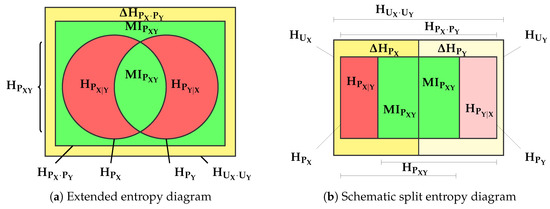
\includegraphics[width=14cm]{Figuras_tfg/ET_Diagram}
  \caption{Diagram representing an ET applied to a bivariate distribution.}
 \label{fig:figure_diagram_et}
\end{figure} 


By applying both equations \ref{eq:normalised_uniformed} and \ref{eq:complex_space_equation} we will get a point in the normalised space  $\Delta'H_{P_{X} * P_{Y}} x 2*MI'_{P_{XY}} x VI'_{P_{XY}}$. Each $P_{XY}$ can be characterised as $F(P_{XY}) = [\Delta'H_{P_{X} * P_{Y}},2*MI'_{P_{XY}},VI'_{P_{XY}}] $. The resulting diagram will be an equilateral triangle, where the coordinates are $F(P_{XY})$ and every bivariate distribution is shown as a point in the diagram. Every zone of the triangle has certain characteristics related to it. \par

We can also divide equation \ref{eq:uniform_entropy_x_y} to obtain new representations of the split balance equations with respect to $X$ and $Y$,

\begin{equation}\label{eq:entropy_x_balance}
H_{U_{X}} = \Delta H_{P_{X}} + MI_{P_{XY}} + H_{P_{X|Y}}  -> 1 = \Delta H'_{P_{X}} + MI'_{P_{XY}} + H'_{P_{X|Y}}
\end{equation}
and,
\begin{equation}\label{eq:entropy_y_balance}
H_{U_{Y}} = \Delta H_{P_{Y}} + MI_{P_{XY}} + H_{P_{Y|X}}  -> 1 = \Delta H'_{P_{Y}} + MI'_{P_{XY}} + H'_{P_{Y|X}}
\end{equation}

Both equations are normalised by using both $H_{U_{X}}$ and $H_{U_{Y}}$ respectibly. Now, we have new representations for $X$ and $Y$ in the 2-simplex triangle created before. The representation seems to split in two and have $F(P_X) = [\Delta'H_{P_{X}},MI'_{P_{XY}},H'_{P_{X|Y}}] $ and $F(P_Y) = [\Delta'H_{P_{Y}},MI'_{P_{XY}},H'_{P_{Y|X}}]$ coordinates.\newline

\begin{figure}[H]
 \centering
  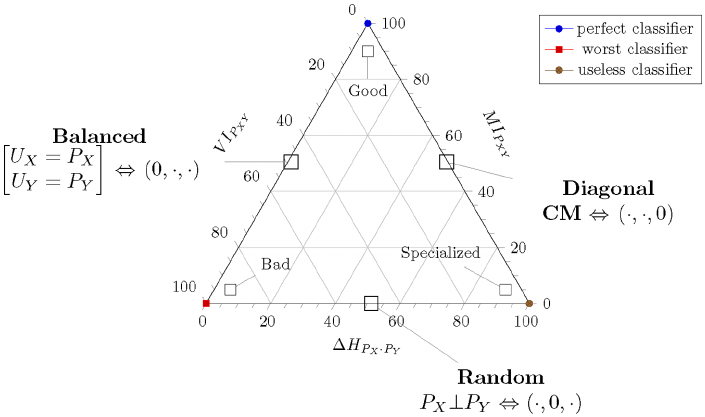
\includegraphics[width=15cm]{Figuras_tfg/ET_Labelled.png}
  \caption{Schematic of an Entropy Triangle. The labels are placed close to the side of the triangle that is related to the feature mentioned in it.}
 \label{fig:figure_labelled_et}
\end{figure} 

Most of the equations included here can be found in [] which discusses most of the points mentioned here along with some examples of use and much more information on the tool and different implications of its use. \par

The triangle itself works as a great tool to characterise the performance of your model. The position of the coordinates assesses the quality of your classifier. It can be appreciated from Figure \ref{fig:figure_labelled_et} that classifiers which are at the apex or close to it obtain the highest accuracy possible on balanced datasets and transmit a lot of mutual information, which makes them the best classifiers possible. On the other hand, when the coordinates of the classifier are very close to the left apex, we will be working with balanced data but the classifier will be doing a very bad work with it, we are dealing with the worst classifier. Finally, those who are located at the right apex or close to it represent the accuracy paradox mentioned before, which a highly specialised classifier which tries to work with very unbalanced data.\par

One example of use of the Entropy Triangle which appears on Section3 together with the results of the experiments would be to use the true labels $K$ and the predicted labels $\hat{K}$ to generate a confusion matrix. Information to be fed the ET can then be calculated with it and thus provide the diagram with enough materials to be created. The tool can then be used for exploratory analysis and help provide visual data to assess the feasibility of the task and its effectiveness.\par

\section{Principal Component Analysis}
\subsection{Description}
The Principal Component Analysis in a statistical procedure based on orthogonal transformations to convert observations of possibly uncorrelated variables into sets of linearly uncorrelated variables called (principal components). The transformation is performed in such a way that the first component has the largest possible variance, with each succeeding component having the highest variance taking into account that it has to be orthogonal to the preceding components. We will finally end up with a set of of vector which are uncorrelated. Due to the nature of the transformation, PCA can be affected by any type of scaling of the original dataset. \par

PCA is used in the data analysis field for exploratory data analysis or to make predictive models. It can be used to visualise the genetic distance between populations of data. Results from the PCA are usually discussed taking into account their components. Other characteristics include:

\begin{description}
	
\item[$\bullet$] PCA is a simple eigenvector-based multivariate analysis. This is specially important to our task since this operation can help us discern the real structure of the data. It can also reduce the dimensionality of the data to view its most informative components and features.

\item[$\bullet$] It resembles factor analysis. Both of them are used to describe the variability of the data and reduce the dimensionality of the data, but aim to use different techniques to reach that goal.

\item[$\bullet$] It also resembles canonical correlation analysis. While CCA tries to describe the cross-variance between two datasets, PCA defines the variance of a single dataset by using an orthogonal coordinate system.

\end{description}

\subsection{PCA and Information Theory}

Our goal when using PCA in this project is to try to give other examples of data transformation to compare the results of the Autoencoder with another widely used tool in the data science field. At the same time, we want the Information theory to be implicit on both methods used so that the outcome can be correctly compared when using the Entropy Triangle.\par

PCA fullfils our requirements by trying to minimise the informational losses. If we assume our model vectors to be defined by the  following equation :

\begin{equation}\label{eq:pca_equation}
x = s + n 
\end{equation}

Where $x$ represents the vector being the sum of the desired information-bearing signal $s$ and a noise signal $n$. If we use this equation, it can be assumed that our vector can be dimensionally reduced.\par

For this model to hold its truth, our signal $n$ has to be Gaussian with a covariance matrix proportional ti the identity matrix. This fact allows us to maximise the mutual information between the dimensionally reduced output $y$ and our $s$ signal, only if we consider that the same assumptions made for $n$ also apply for $s$. \par

On the other common scenarios, on which $s$ is not Gaussian, at least we will have an upper-bound for our representation such as,

\begin{equation}
\label{eq:pca_upper_bound}
I(x;s) - I(y;s)
\end{equation}

If our noise is dependant, the PCA losses its informational properties and thus we cannot use the previous representations. On the other hand, if our noise is more Gaussian that our bearing signal $s$, our PCA representation will be optimal.


\section{The classifiers}
\subsection{Knn}

Knn is a non-parametric supervised classification method used for estimating the density function. As an unsupervised algorithm, it needs labelled data to learn the appropriate function that produces new data belonging to the different regions of the existing classes when introducing new unlabelled data. Depending on the desired predictors we will want to obtain either a regression or a discrete output in our classifier. \par

The Knn algorithm hinges on the assumption that similar data must be close. This theory means that, in practice, we must take into account that proximity will be primordial to the outcome of our classification process when we are using the Knn classifier. This particular way of solving a data analysis problem is specially interesting when the data we are trying to analyse is very close to the same labelled data. \par

Although "the majority voting" classification method has some positive advantages, it also comes with some drawbacks too. In case where the class distributions are skewed, we can end up with a class which solely dominates the predictions. The are many ways of overcoming this issue, such as assigning proportional weights or to build clusters with similar points, but the reality is that Knn has a defined scalability that depends on the noise of your data and the characteristic of your dataset. \par

In order to try to improve results and polish the overall performance of the algorithm. There are some tricks to take into account and try to follow when designing it: \par

\begin{description}
	
\item[$\bullet$] Try fitting your data through multiple instance of your implemented algorithm with new values for K in each case.

\item[$\bullet$] Avoid using even K's values when doing binary classification, as we want to avoid tied votes.

\item[$\bullet$] Perform an exploratory analysis of your data and design the boundaries and expected performance of your algorithm. Sometimes, realising that a problem will be very lengthy and tedious to solve using a pre-determined method will save you a lot of time .

\end{description}

\begin{figure}[H]
\centering
  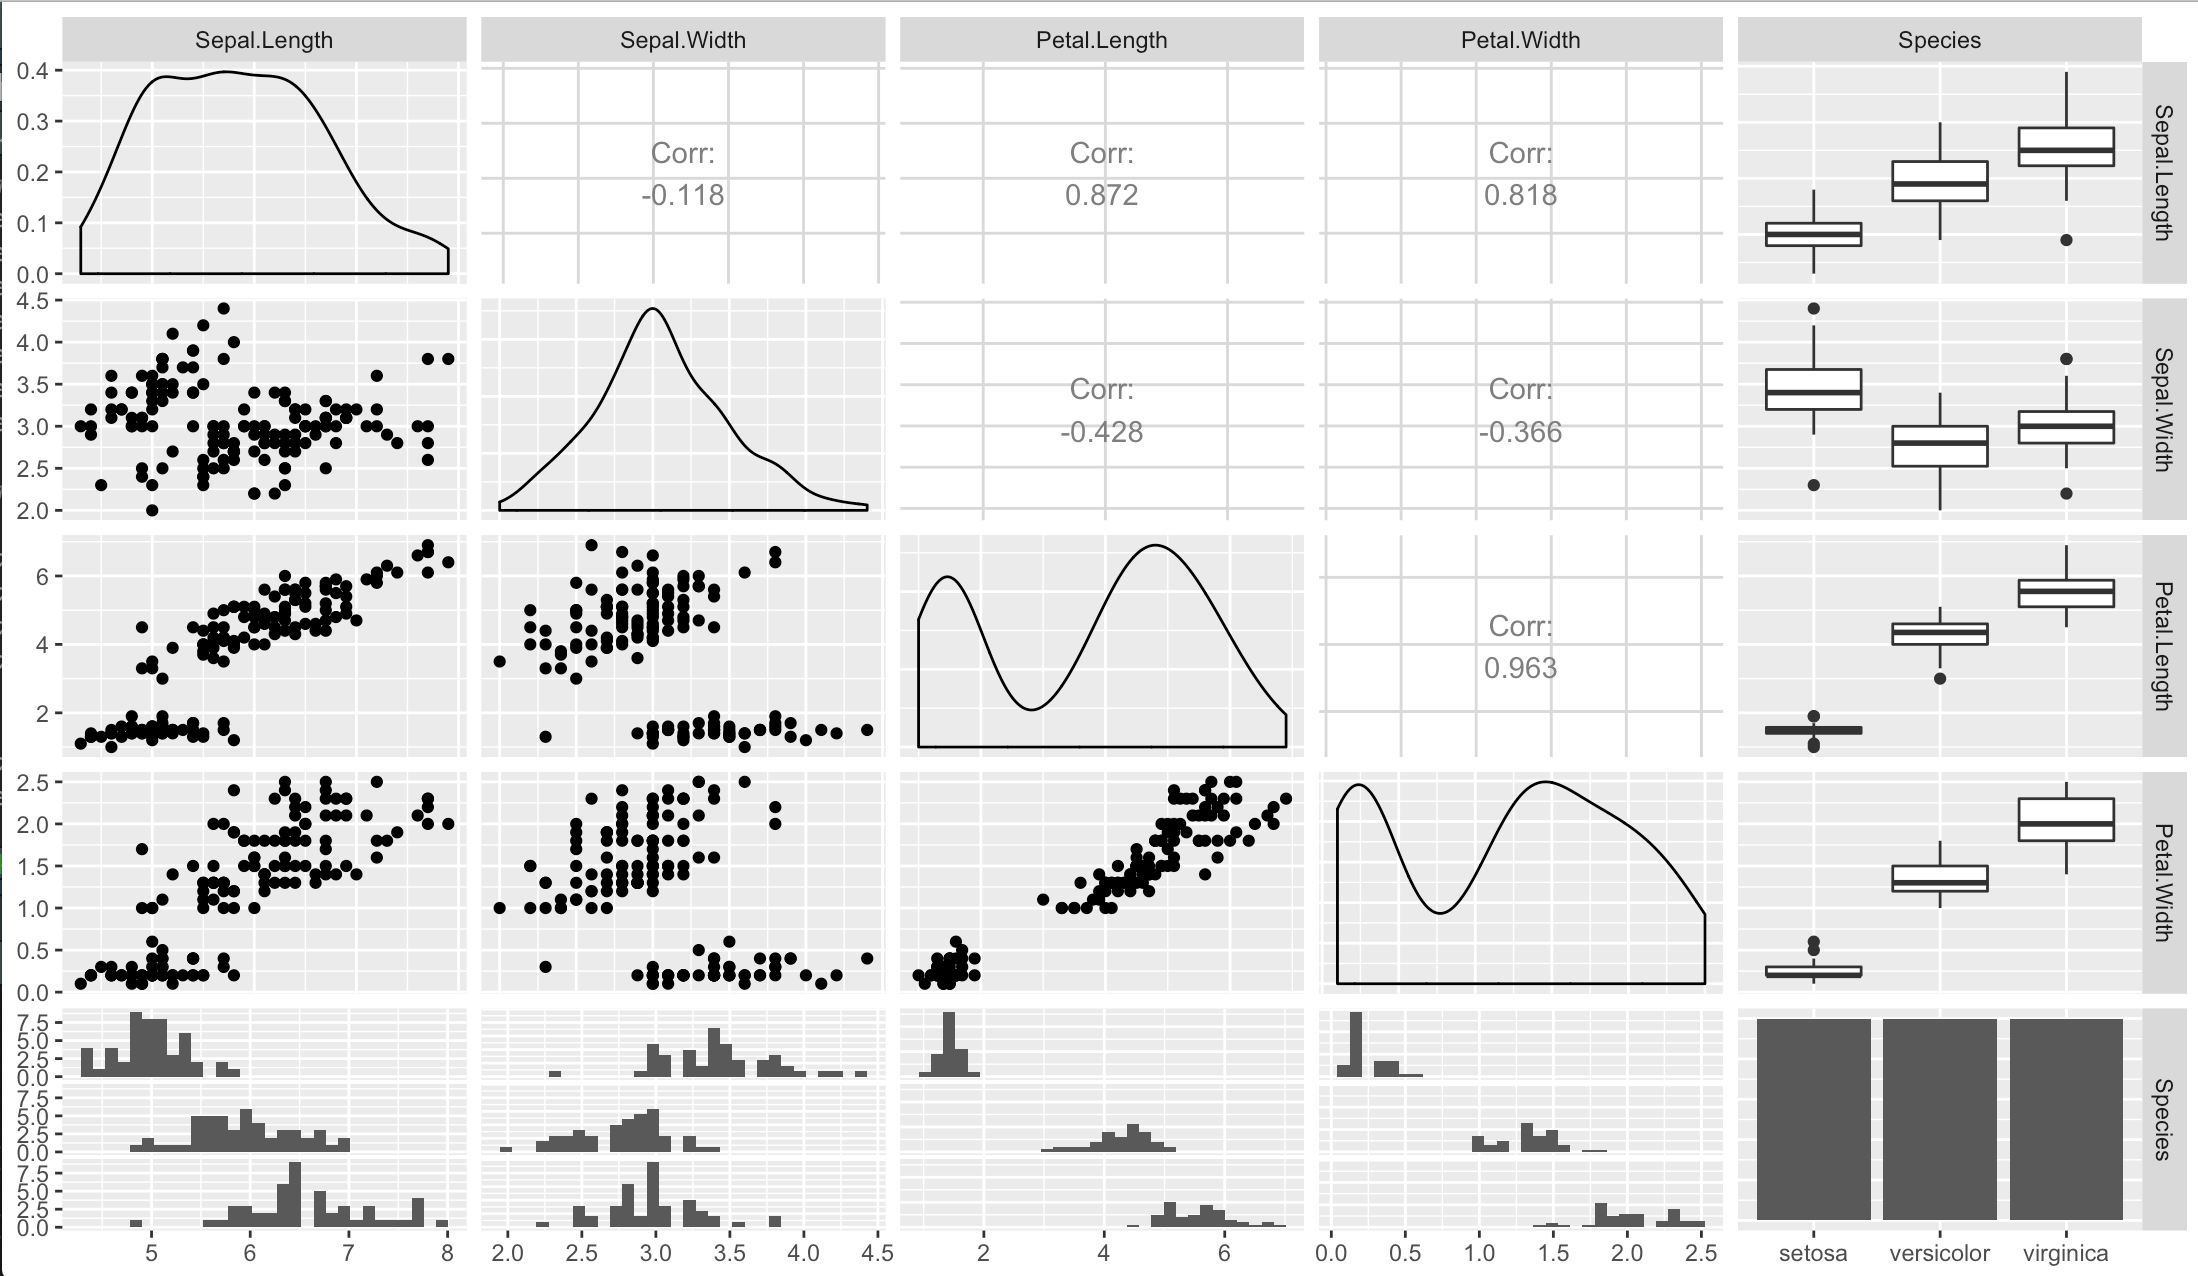
\includegraphics[width=15cm]{Figuras_tfg/R_plot_correlation.png}
  \caption{The GGally package also provides useful tools for this types of problems. Here, the correlation between Petal.Length and Petal.Width is proven to be very high, as the plots from Figure \ref{fig:figure_knn_classifier}}
 \label{fig:figure_knn_classifier_correlation}
\end{figure}

\subsection{Multilayer Perceptron}

The Multilayer Perceptron(MLP) has a similar architecture to that of the Deep Neural Networks. Both of them have input, output and hidden layers as well as having nodes and backpropagation for training. They even need their layers to be activated, as well as support the most common functions used in the autoencoders. Some experts would even label it as a slightly less computationally powerful DNN. \par

It would seem as the main interest into MLPs could be to use them for smaller Autoencoders, but actually they possess a very important feature: it can distinguish and classify data that is not linearly separable.This property can help us qualify and compare different types of classification tasks. And as it is interesting to test multiple algorithms to make the most out of our ET, we can use it together with the rest of the classifiers presented in this Section. It can be specially useful when we pair it with the knn classifier, as we will implement both of them in our project to perform the same tasks. We would expect it to generally perform better on more complex datasets than knn, which suffers when data is more difficult to differentiate. \par
